\cohead{\Large\textbf{Integrationsgrenze bestimmen}}
\fakesubsection{Bestimmen von Integrationsgrenzen}
Eine des Öfteren vorkommende Aufgabenstellung beinhaltet das grafische Abschätzen oder das Berechnen einer Integrationsgrenze. Bei diesem Aufgabentyp ist in der Regel die obere Integrationsgrenze gesucht.\\
Beispiel: Gegeben ist das Schaubild der Funktion \(f(x)\). Gesucht sind zwei Lösungen \(u>0\), so dass \(\int_0^u f(x) \td x=0\) gilt.\\ \\
\begin{minipage}{\textwidth}
	\adjustbox{valign=t}{\begin{minipage}{.5\textwidth}\raggedright
		Grafische Abschätzung:\\
		\textcolor{loes}{Damit der Wert des Integrals Null ergibt, müssen die Teilflächen oberhalb der \(x\)-Achse und unterhalb der \(x\)-Achse gleich groß sein. Dies ist für \(x_1\approx 1\) und \(x_2\approx 4\) der Fall, wie man sehen kann, wenn man die entsprechenden Flächen im Schaubild markiert.}\\
	\end{minipage}}
	\adjustbox{valign=t}{\begin{minipage}{.5\textwidth}
		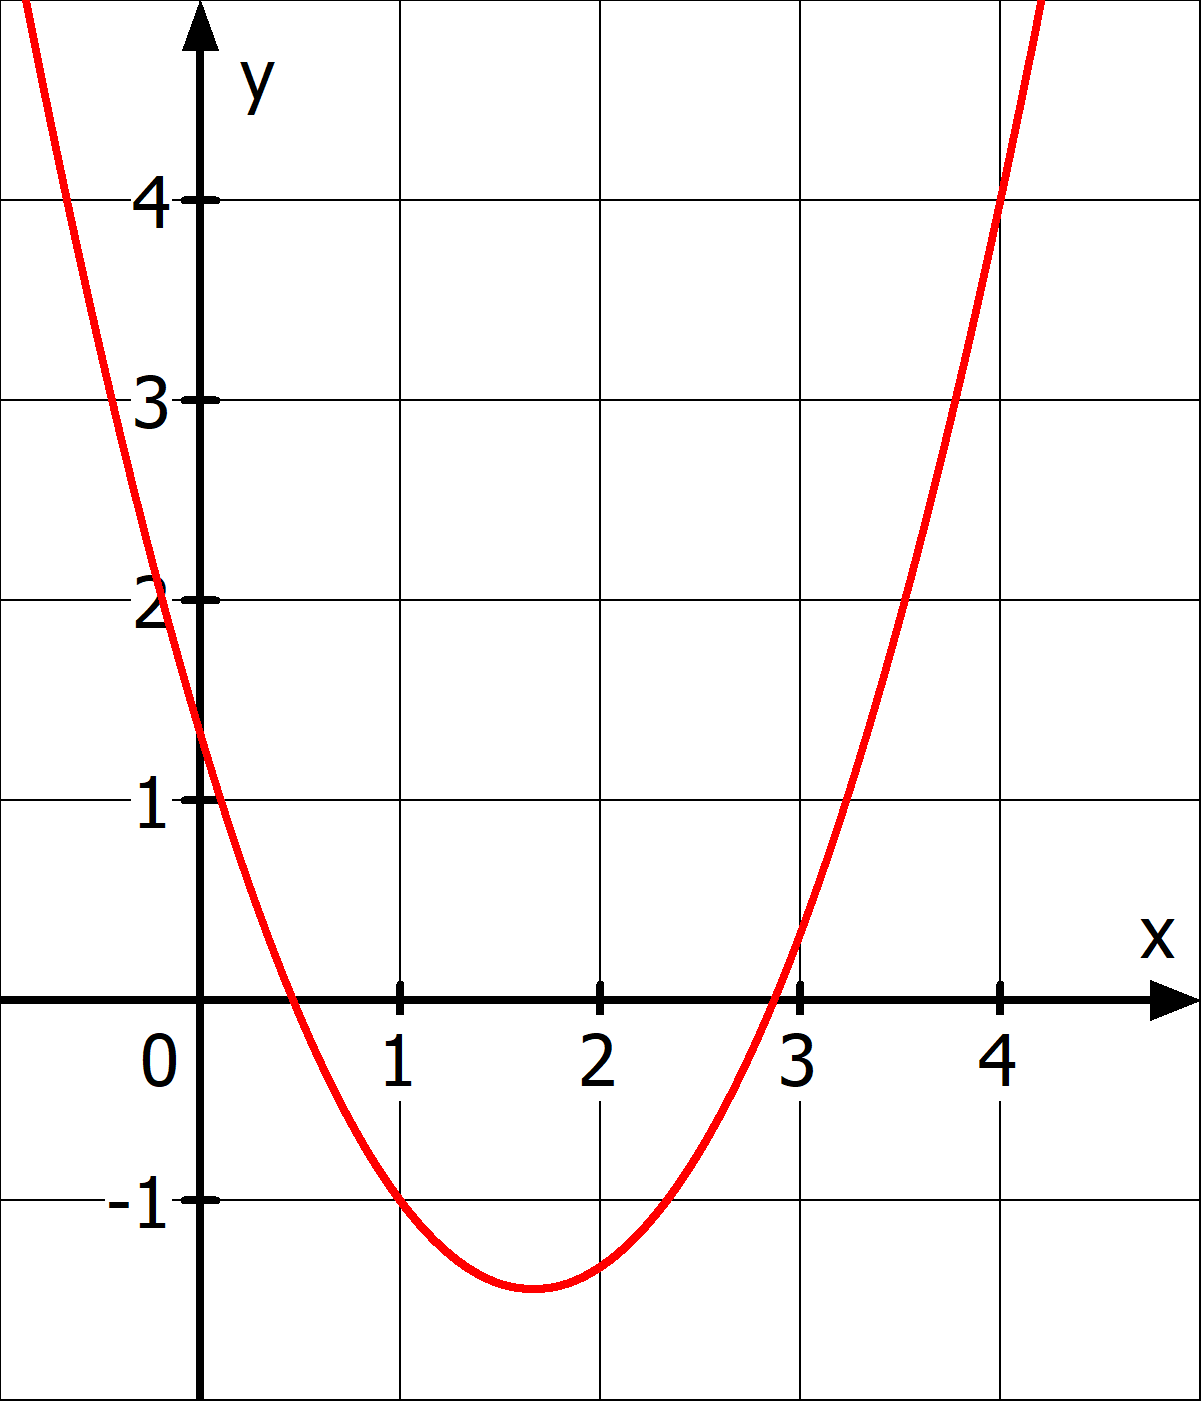
\includegraphics[width=.95\linewidth]{\integration/pics/grenzeBsp1.png}
	\end{minipage}}
\end{minipage}\vspace{\baselineskip}\\
Ist die Funktionsgleichung bekannt, so kann man die Lösung auch berechnen. Im Beispiel ist \(f(x)=x^2-\frac{10}{3}x+\frac{4}{3}\):\\
\textcolor{loes}{Wir lösen die oben gegebene Gleichung:}
\begin{align*}
	\textcolor{loes}{\int_0^u f(x) \td x}&\textcolor{loes}{=0}\\
	\textcolor{loes}{\int_0^u x^2-\frac{10}{3}x+\frac{4}{3} \td x}&\textcolor{loes}{=0}\\
	\textcolor{loes}{\left[\frac{1}{3}x^3-\frac{5}{3}x^2+\frac{4}{3}x \right]_0^u}&\textcolor{loes}{=0}\\
	\textcolor{loes}{\frac{1}{3}u^3-\frac{5}{3}u^2+\frac{4}{3}u}&\textcolor{loes}{=0}\\
	\textcolor{loes}{u\left(\frac{1}{3}u^2-\frac{5}{3}u+\frac{4}{3}\right)}&\textcolor{loes}{=0}\\	
	\textcolor{loes}{\text{S.v.N.: }u_0=0\text{ oder }\frac{1}{3}u^2-\frac{5}{3}u+\frac{4}{3}}&\textcolor{loes}{=0}
\end{align*}
\textcolor{loes}{Die Mitternachtsformel liefert \(u_1=1\) und \(u_2=4\). Da laut Aufgabenstellung \(u>0\) sein soll, sind nur \(u_1\) und \(u_2\) zulässige Lösungen.}
\newpage

\begin{Exercise}[title={\raggedright\normalfont Schätze jeweils ein \(u\) graphisch ab und berechne dann die Lösung. Das gesuchte \(u\) soll immer größer als die untere Grenze sein:}, label=intGrenzeA1]\\
	\begin{minipage}{\textwidth}
		\begin{minipage}{.5\textwidth}
			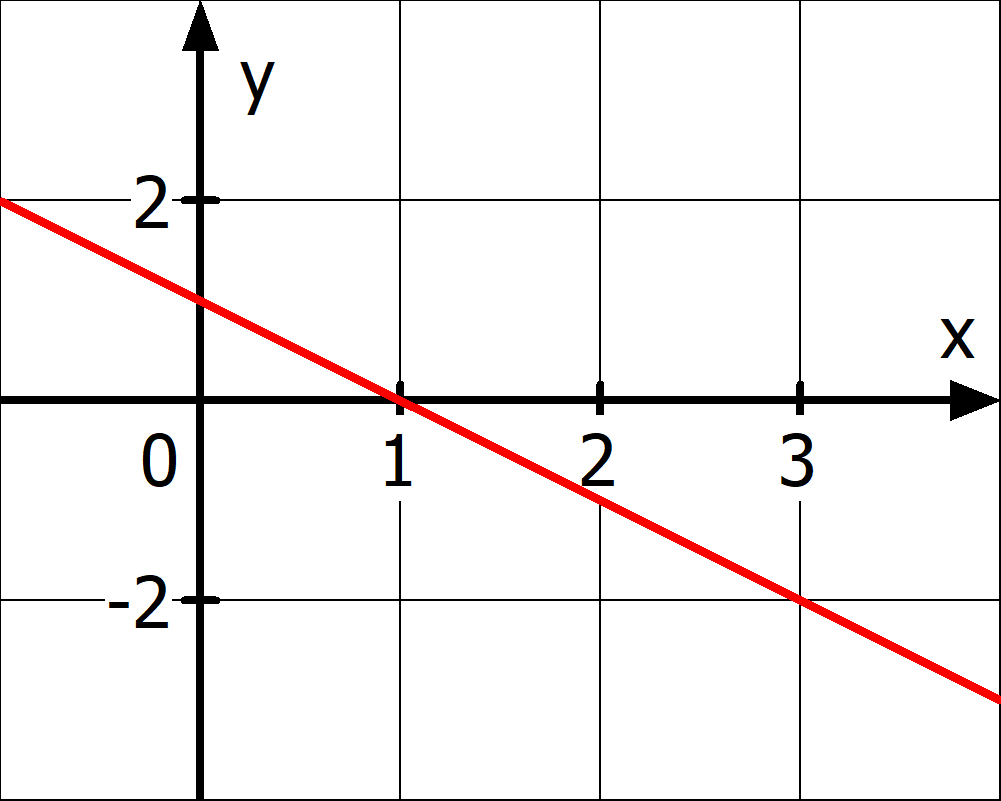
\includegraphics[width=.8\linewidth]{\integration/pics/intGrenze1.png}
			\[\int_0^u-\tfrac{1}{2}x+\tfrac{1}{2} \td x=-1\]
		\end{minipage}
		\begin{minipage}{.5\textwidth}
			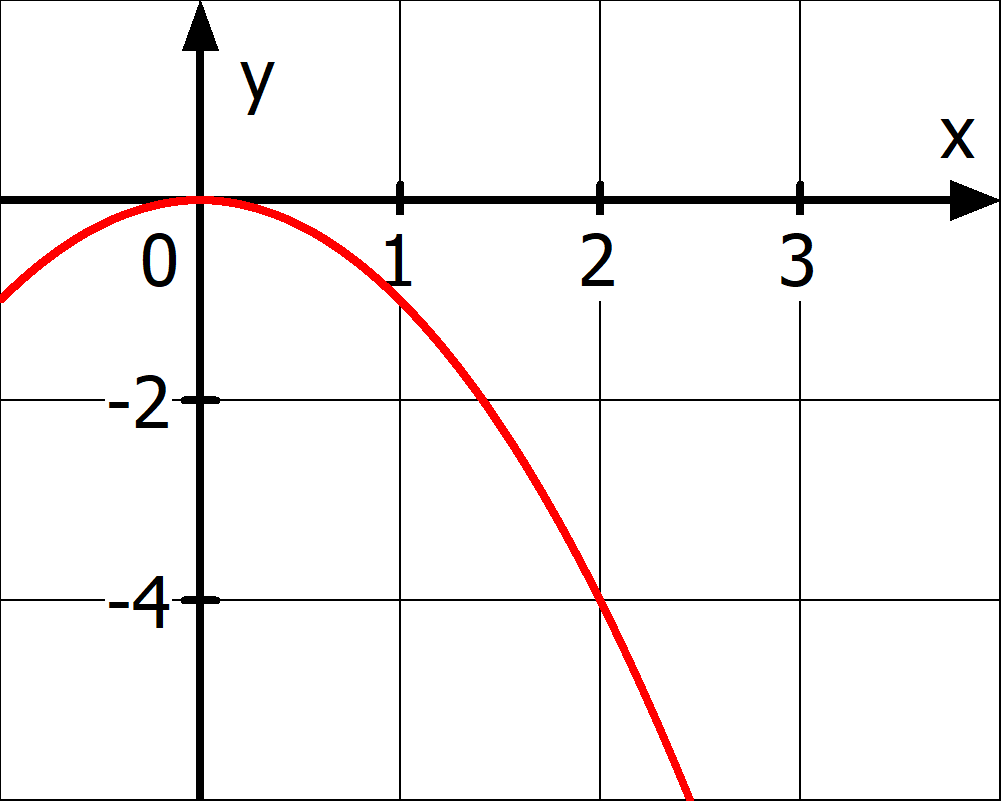
\includegraphics[width=.8\linewidth]{\integration/pics/intGrenze2.png}
			\[\int_{-1}^u-0,5x^2 \td x=-1,5\]
		\end{minipage}\vspace{\baselineskip}\\
		\begin{minipage}{.5\textwidth}
			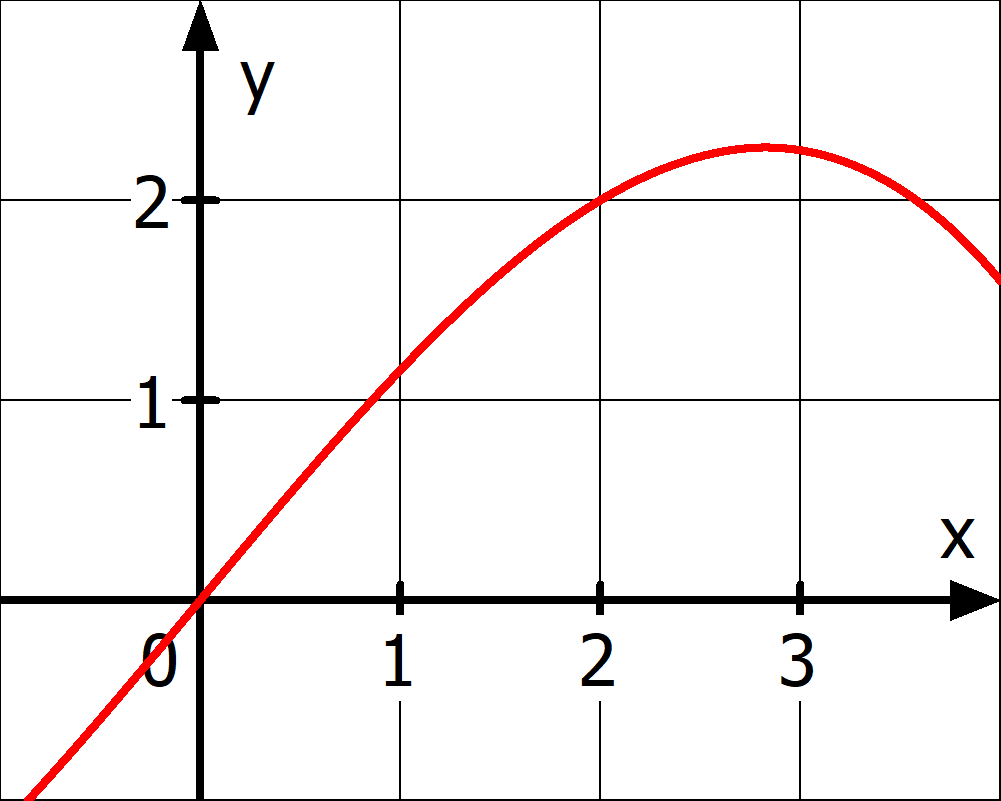
\includegraphics[width=.8\linewidth]{\integration/pics/intGrenze3.png}
			\[\int_0^u-\tfrac{1}{20}x^3+\tfrac{6}{5}x \td x=2,2\]
		\end{minipage}
		\begin{minipage}{.5\textwidth}
			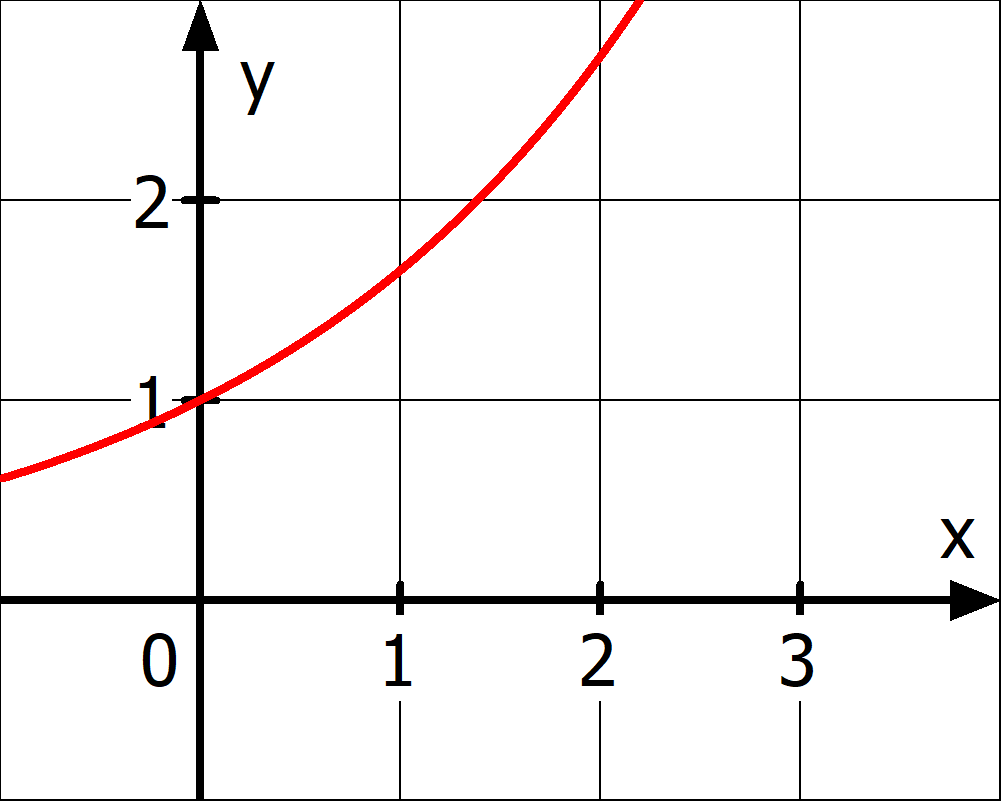
\includegraphics[width=.8\linewidth]{\integration/pics/intGrenze4.png}
			\[\int_0^u e^{0,5x} \td x=4\]
		\end{minipage}\vspace{\baselineskip}\\
		\begin{minipage}{.5\textwidth}
			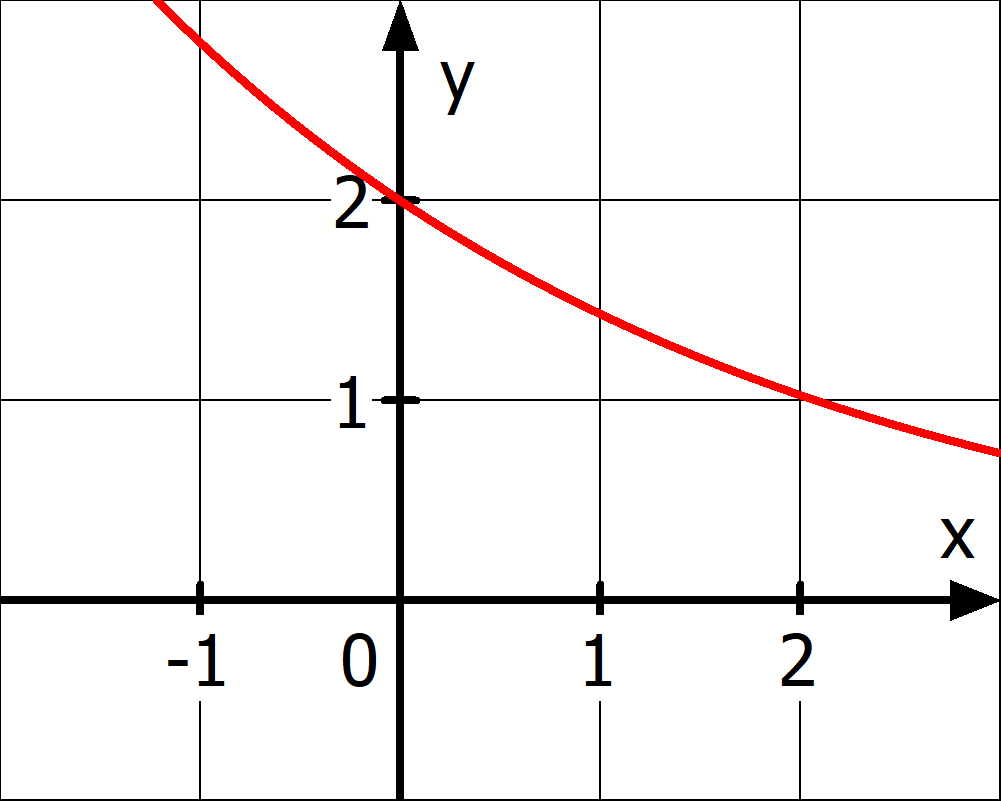
\includegraphics[width=.8\linewidth]{\integration/pics/intGrenze5.png}
			\[\int_{-1}^u 2e^{-\tfrac{1}{3}x} \td x=5\]
			\phantom{Finde 2 verschiedene \(u>0\).}
		\end{minipage}
		\begin{minipage}{.5\textwidth}
			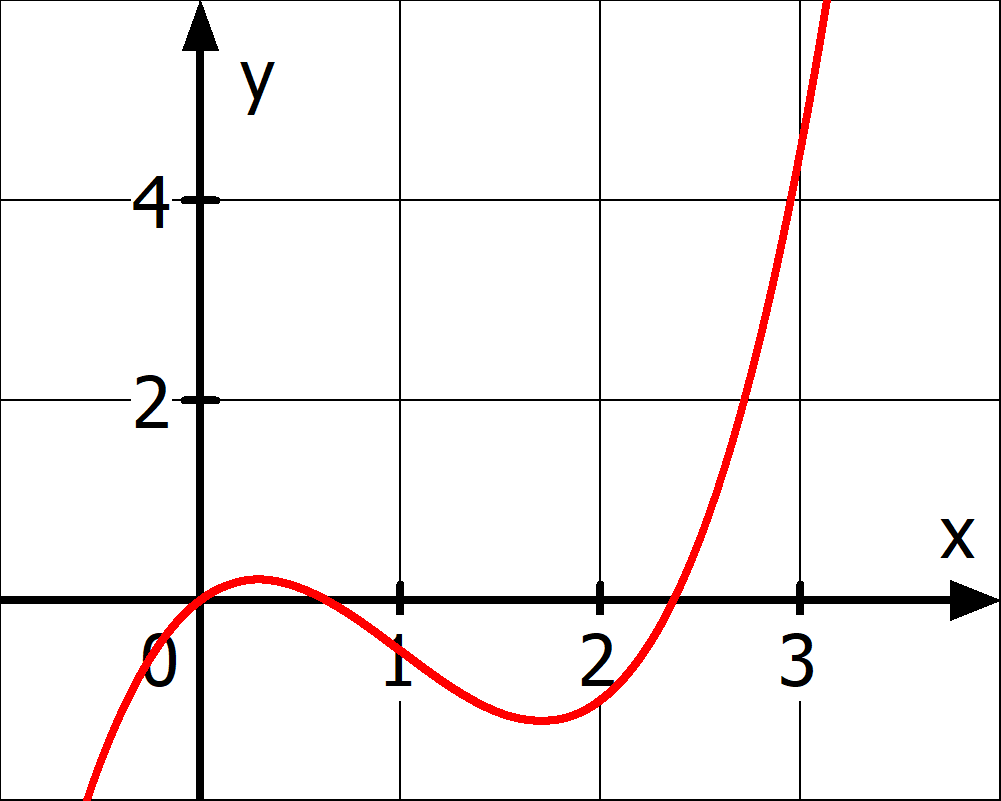
\includegraphics[width=.8\linewidth]{\integration/pics/intGrenze6.png}
			\[\int_0^u \tfrac{1}{2}x^3-\tfrac{3}{2}x^2+\tfrac{3}{4}x \td x=0\]
			\centering{Finde 2 verschiedene \(u>0\).}
		\end{minipage}
	\end{minipage}
\end{Exercise}

%%%%%%%%%%%%%%%%%%%%%%%%%%%%%%%%%%%%%%%%%
\begin{Answer}[ref=intGrenzeA1]\\
	Die grafisch abgeschätzten Lösungen sollten jeweils bis auf \(\pm0,3\) mit den berechneten Lösungen übereinstimmen. Lösungen in Klammer lösen zwar die Gleichung, sind aber nicht größer als die untere Grenze.\\
	\begin{minipage}{\textwidth}
		\begin{minipage}{.5\textwidth}\raggedright
			\[\int_0^u-\frac{1}{2}x+\frac{1}{2} \td x=-1\]
			\[u_1=1+\sqrt{5}\approx3,24\ \left(\text{und }u_2=1-\sqrt{5}\right)\] 
		\end{minipage}
		\begin{minipage}{.5\textwidth}
			\[\int_{-1}^u-0,5x^2 \td x=-1,5\]
			\[u_1=2\]
		\end{minipage}\vspace{\baselineskip}\\\vspace{\baselineskip}\\
		\begin{minipage}{.5\textwidth}\raggedright
			\[\int_0^u-\tfrac{1}{20}x^3+\tfrac{6}{5}x \td x=2,2\]
			\[u_1=2, u_2=\sqrt{44}\ \left(\text{und }u_3=-2,\ u_4=-\sqrt{44}\right)\]
		\end{minipage}
		\begin{minipage}{.5\textwidth}
			\[\int_0^u e^{0,5x} \td x=4\]
			\[u_1=2\ln(3)\]
		\end{minipage}\vspace{\baselineskip}\\\vspace{\baselineskip}\\
		\begin{minipage}{.5\textwidth}\raggedright
			\[\int_{-1}^u 2e^{-\tfrac{1}{3}x} \td x=5\]
			\[u_1=-3\ln\left(e^{\tfrac{1}{3}}-\frac{5}{6}\right)\]
		\end{minipage}
		\begin{minipage}{.5\textwidth}
			\[\int_0^u \frac{1}{2}x^3-\frac{3}{2}x^2+\tfrac{3}{4}x \td x=0\]
			\[u_1=1,\ u_2=3\ \left(\text{und }u_3=0\right)\] 
		\end{minipage}
	\end{minipage}
\end{Answer}